\section{Papers and Applications}

\subsection{AGU abstract: What limits fire, where and when: sensitivity of burnt area to different controls}

\subsubsection{Abstract}
Global fire models typically describe fire as a consequence of fuel load, moisture, natural and anthropogenic
ignitions, and land use suppression. A lack of information on the temporal and spatial distribution of these
controls has meant that their simulated effects on predicting burnt area are largely untested. Despite this,
there is a pervasive assumption that burnt area is proportional to the number of ignitions, with many models
predicting significant increases in burnt area with human fire starts.


Here, we map the limitation and sensitivity of burnt area to each control using a simple framework whereby
limitations are imposed by: fuel discontinuity; fuel moisture and atmospheric drying potential; lightning and
human ignitions; and land use. Limitations are described from remote sensed and meteorological
observations and optimized against Global Fire Emissions Database (GFED4s) burnt area observations.
Fuel moisture is shown to be the main limitation of fire over much of the world, (44\% annual average and
36\% during local dry seasons), particularly in the humid forests and cold, slow drying boreal areas. Fuel
discontinuity is the next limitation (25\% annually and 23\% in the dry season), especially in deserts and dry
season grasslands. This is followed by land use change (18\% annually, 21\% dry season) and then ignitions
(13\% annually, 19\% dry season), which is only a significant limiting factor in dry season savanna, where
rapid drying of fuel built up during the wet season removes all other natural limitations. In these areas,
changes in burnt area are actually more sensitive to other controls, typically land use.


This study contradicts the way basic processes are represented in many global fire models. As ignitions only
impact burnt area over a limited geographic extent, better representation of controls imposed by fuel loads
and moisture is vital. Human ignitions only contribute to a small increase in global burnt area (2\%), which is
offset by the dramatic impact of suppression through anthropogenic land cover changes. The assumption
that humans cause burnt area over much of the world is therefore clearly incorrect, and adequate simulation
of suppression through land use should become a priority. This result also has implications when considering
ecosystem services of agricultural land and fire management policies.

\pagebreak
x
\pagebreak
\subsection{Anthropagenic regime shifts}
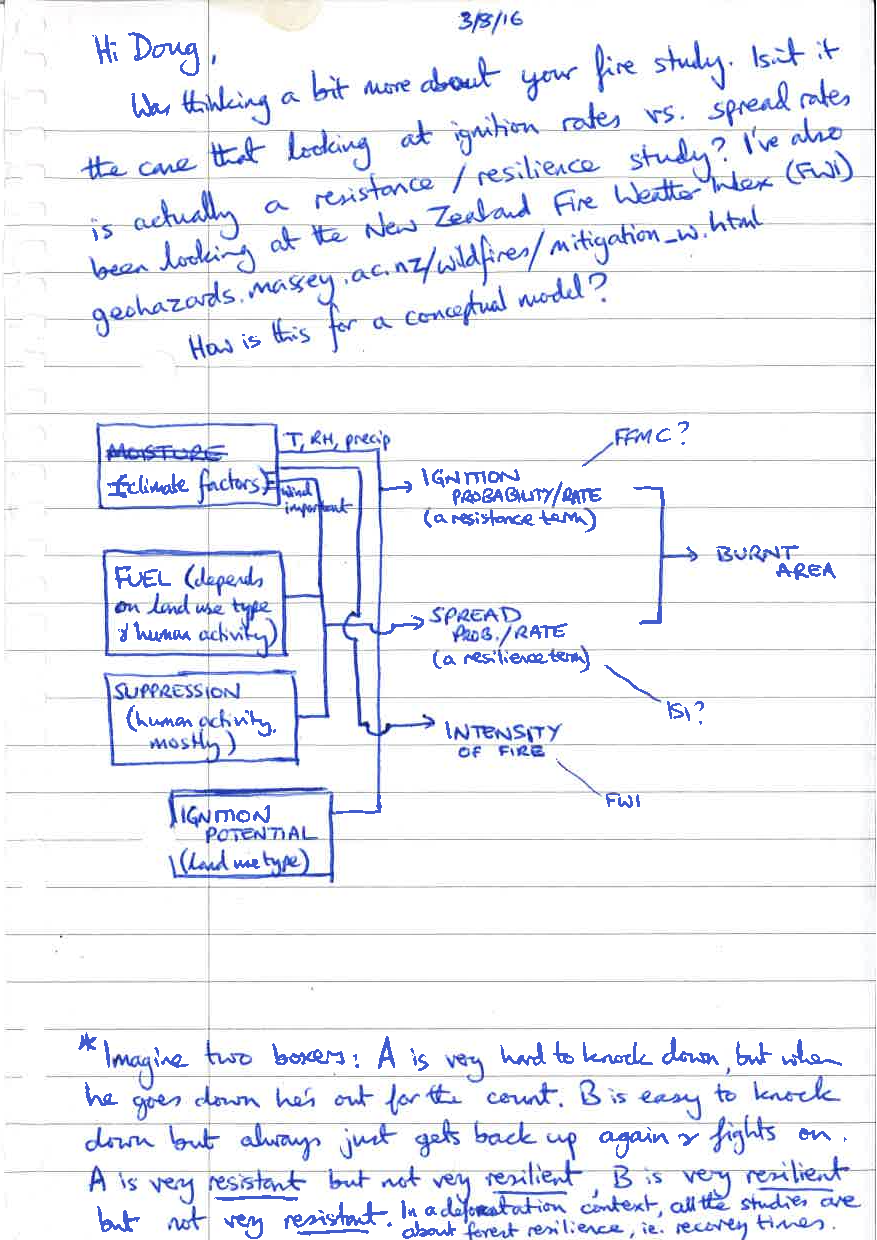
\includegraphics[width=0.99\textwidth]{diagrams/tobys_notes.pdf}
